%File Name:data_stu.tex
%Created Time: 2019-07-12 10:28:19 week:5
%Author: hanhj
%Mail: hanhj@zx-jy.com 
\documentclass{article}
\usepackage{xeCJK}
\usepackage{indentfirst}
\usepackage{listings}
\usepackage{graphicx}
\usepackage{makeidx}
\usepackage[breaklinks,colorlinks,linkcolor=black,citecolor=black,urlcolor=black]{hyperref}
\setCJKmainfont{AR PL UMing TW MBE}
\makeindex
\lstset{language=C}
\begin{document}
%\begin{xeCJK}{UTF8}{gbsn}
\title{数据结构学习}
\author{hanhj}
\maketitle
\newpage
\tableofcontents
\newpage
\section{绪论}
\subsection{算法概念}
	\par
	算法是为利用计算机来解决实际问题,而所进行的设计和实现的方法。
	\par
	问题=》算法=》程序实现。\\
	\par
	性质:
	\begin{itemize}
		\item 有输入
		\item 有输出
		\item 唯一性
		\item 有穷性
	\end{itemize}	
	\par
	步骤:
	\begin{enumerate}
		\item 分析问题:输入,输出,要求
		\item 数据结构设计
		\item 算法设计:策略,方法
		\item 算法分析
		\item 程序实现 
	\end{enumerate}
			
\subsection{渐近性分析}
\subsection{递归的渐近性分析}
\section{线性表}
\subsection{线性表}
\subsubsection{线性表的存储与操作}
\subsubsection{栈}
\subsubsection{队列}
\subsection{查找}
\subsection{排序}
\section{递归与分治}
\section{二叉树}
	\subsection{树的定义}
		线性表中的每个中间节点,都只有一个前驱和一个后继。而对于树而言,每个中间节点都只有一个前驱,但有多个后继。特别的如果有两个后继,称为二叉树。

	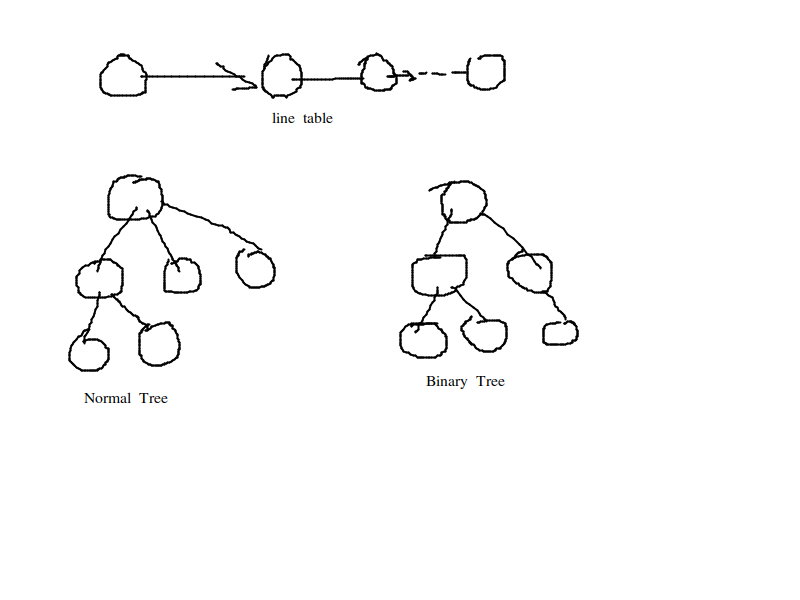
\includegraphics[scale=0.4]{./pic/tree-01.png}

	\textbf{二叉树的形态:}
	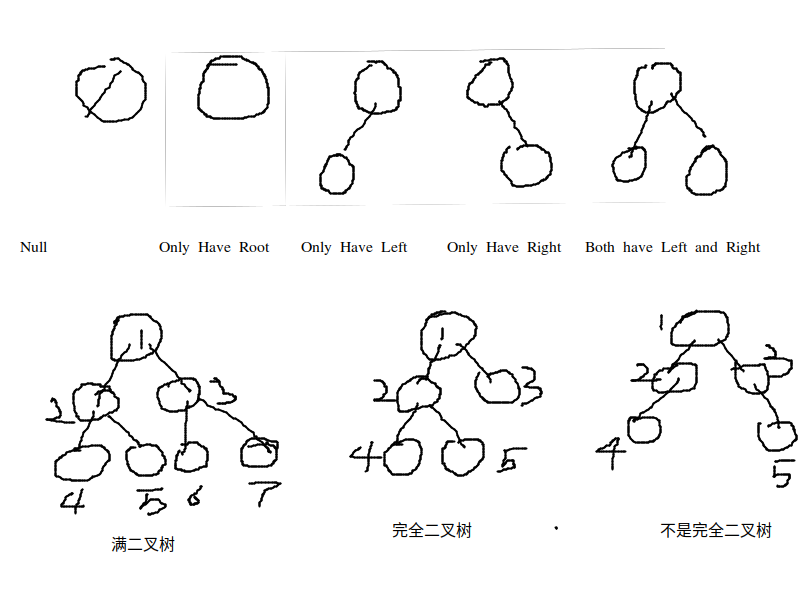
\includegraphics[scale=0.4]{./pic/tree-02.png}
	
	按照从上到下,从左到右完全二叉树的节点编号应当与满二叉树编号一致。

	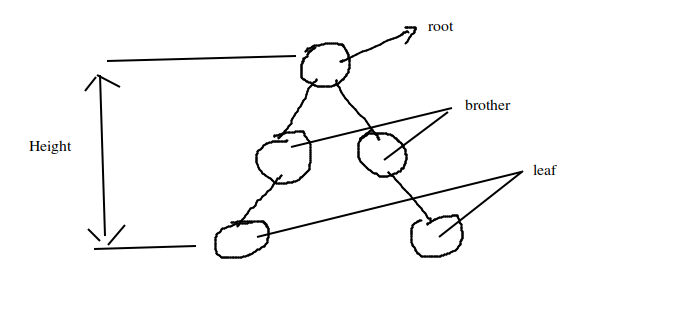
\includegraphics[scale=0.4]{./pic/tree-02-1.png}

	度是指节点的孩子数。

	\textbf{二叉树的存储}

	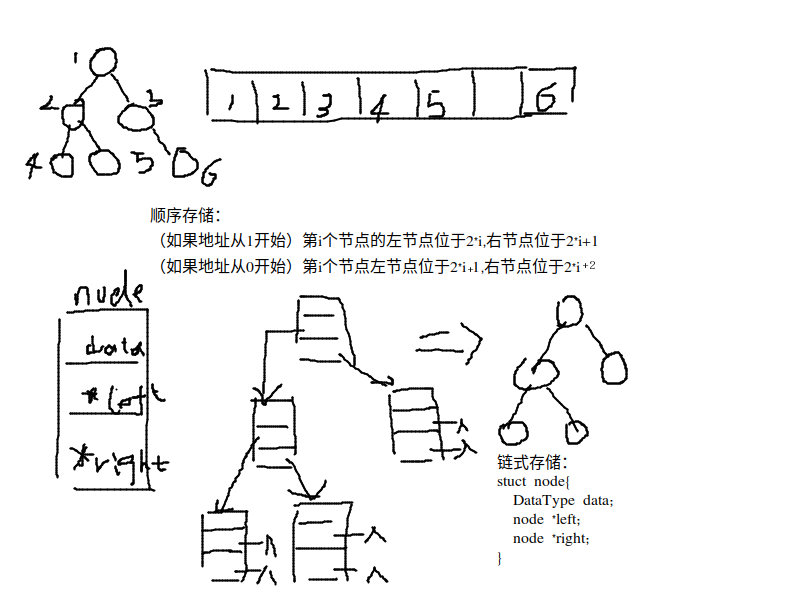
\includegraphics[scale=0.4]{./pic/tree-03.png}

	如果用顺序存储,则k层的二叉树需要$2^{k}-1$个内存,如果是稀疏二叉树,则空间浪费比较严重。

	\textbf{二叉树的性质:}
	\begin{enumerate}
		\item 每层的节点数最多为$2^{k-1}$个。
		\item k层二叉树最多节点数$2^{k}-1$个
		\item 叶子节点数=度为2的节点树+1。即n0=n2+1
			\begin{verbatim}
				证明:
				N=n0+n1+n2
				从分支数而言,每个分支对应一个节点
				N=2*n2+n1+1 1是根节点
				所以:
				n0=n2+1
			\end{verbatim}
		\item 对完全二叉树而言,高度:$Height=\lfloor log_2N \rfloor $
	\end{enumerate}
	\subsection{二叉树的遍历}
		先根遍历:对于每个节点按照TLR顺序遍历,即先访问根再递归访问左子树,再递归访问右子树。

		中根遍历:对于每个节点按照LTR顺序遍历,即先递归访问左子树,再访问根,再递归访问右子树。

		后根遍历:对于每个节点按照LRT顺序遍历,即先递归访问左子树,再递归访问右子树,再访问根。

		层次遍历:按照层次遍历每一层的节点。

		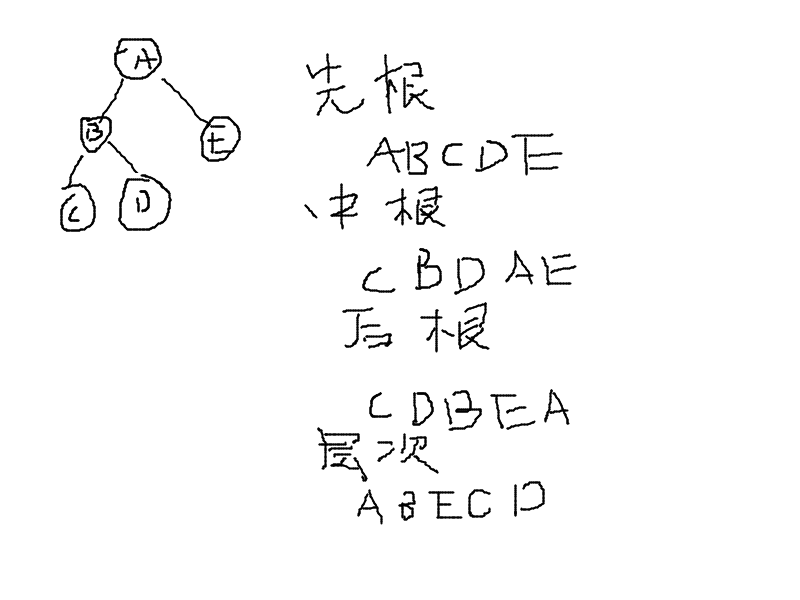
\includegraphics[scale=0.4]{./pic/tree-04.png}

		\begin{verbatim}
    void _pre_order(BiNode<T> *node){
      if(node==NULL)
        return;
      visit(node);
      _pre_order(node->left);
      _pre_order(node->right);
    }
    void _in_order(BiNode<T> *node){
      if(node==NULL)
        return;
      _in_order(node->left);
      visit(node);
      _in_order(node->right);
    }
    void _back_order(BiNode<T> *node){
      if(node==NULL)
        return;
      _back_order(node->left);
      _back_order(node->right);
      visit(node);
    }
   void level_order(BiNode<T>*node){
      if(node==NULL)
         return;
      queue<T*> q;
      q.push(node);
      T *p;
      while(q.empty()!=true){
         p=q.front();
         q.pop();
         visit(p);
         if(p->left){
            q.push(p->left);
         }
         if(p->right){
            q.push(p->right);
         }
      }
   }
		\end{verbatim}

		对于中序遍历,其值是非递减顺序排列的。


		\textbf{根据遍历恢复二叉树}

		通过一个遍历结果不能恢复二叉树,只有通过两个遍历结果才能恢复二叉树。

		假设现在有先根和中根遍历结果:ABCDE,CBDAE。

		在先根遍历中取第一个根A,然后在中根遍历中找到A,其左边为左子树(CBD),右边为右子树(E)。

		然后在先根遍历中取第二个根B,然后在中根遍历的左子树中找到B,其左边为左子树(C),右子树为(D)。这样就完成了B的恢复,同时也完成了A的左子树的恢复。

		再看A的右子树,只有E,这样就完成了A的右子树的恢复。也同时完成了A的恢复。
		
		代码如下:
		\begin{verbatim}
    /*
    pre_ord :pre_order data array
    in_ord :in_order data array
    l,r pre_order data array start and end pos
    k,h in_order data array start and end pos
    root : return node
    */
    int _create_tree(T*pre_ord,T*in_ord,int l,int r,int k,int
        h,BiNode<T> *& root){
      int m;
      BiNode<T>*node;
      node=new BiNode<T>;
      if(node==NULL)
        return -1;
      node->data=pre_ord[l];
      root=node;
      m=k;
      while(m<=h && pre_ord[l]!=in_ord[m])
        m++;
      if(m==k){//node havn't left tree
        node->left=NULL;
      }else{//build left tree
        _create_tree(pre_ord,in_ord,l+1,l+m-k,k,m-1,(root)->left);
      }
      if(m==h){//node have not right tree
        node->right=NULL;
      }else{//build right tree
        _create_tree(pre_ord,in_ord,l+m-k+1,r,m+1,h,(root)->right);
      }
      return 0;
    }
		\end{verbatim}
	\subsection{排序二叉树Binary Sort Tree(BST)}
		将比当前节点值小的节点放在当前节点左边,比当前节点值大的节点放在当前节点的右边。称为BST。在BST中查找的时间复杂度平均为$O(nlogN)$
		\subsubsection{BST的查找}
		\subsubsection{BST的插入与删除}
	\subsection{平衡二叉树AVL}
		\subsubsection{AVL的插入与删除}
	\subsection{哈夫曼树}
		叶子节点的路径长度:是指从根节点到叶子节点边的数目。$L_i$

		叶子节点的带权路径长度:是指叶子节点的路径长度乘以叶子节点的权。$W_i*L_i$

		树的路径长度:是指树中所有叶子节点的路径长度之和。$\sum^{n}_{i=1}{L_i}$

		树的带权路径长度:是指树中所有叶子节点的带权长度之和。$WPL=\sum_{i=1}^{n}{W_i*L_i}$

		哈夫曼树是一种带权树,其树的带权长度最小。

		哈夫曼树的构造是从当前节点中选取两个最小权值的点组合成一个新点,同时删除原叶子节点中的这两个点,该新点加入到待构造的节点中,然后递归的执行这个步骤。可以证明,哈夫曼树的带权路径长度最小。

		\textbf{哈夫曼编码}

		对于数据我们通常对其进行编码,比如常用的ascii编码,gbk编码,都是用等长的位对数据进行编码。ascii是8位,gbk是16位。哈夫曼编码是为了减少数据传输过程中的数据的长度,对数据采用不等长编码。对于使用频度较大的数据采用较短的位,对于使用频度较大的数据采用较长的位。同时,还要能够从数据流中恢复数据,保证能够区分各个数据。

		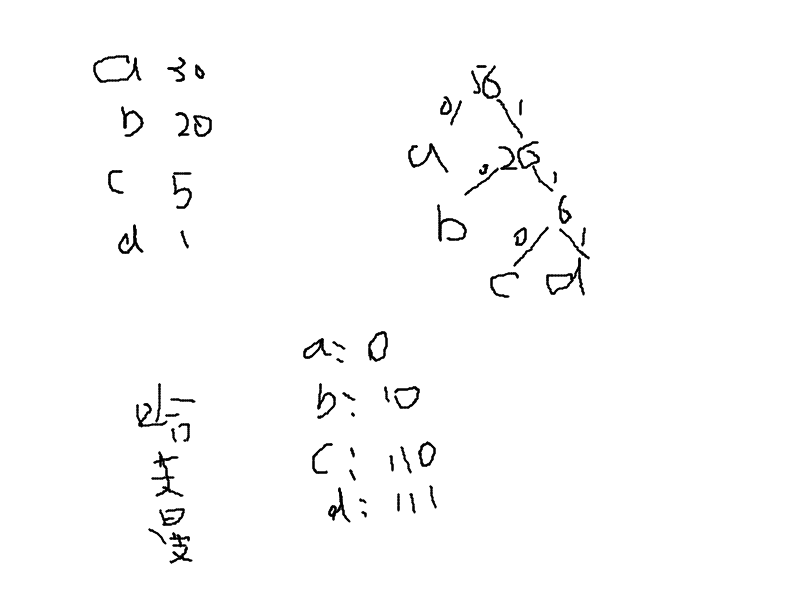
\includegraphics[scale=0.4]{./pic/tree-05.png}

		字符abcd的频度如上所示,按照频度构造一个哈夫曼树,然后将左边标记为0,右边标记为1,对于叶子节点的编码就是其路径上的数字。经过哈夫曼编码后可见出现频度高的a编码最短,频度低的编码较长。

	\subsection{堆}
		
		堆是一个数组,其中的任何元素:
		\[
			A_{i}<
				\left\{
					\begin{array}{ll}
						A_{2*i} & \textbf{小顶堆}\\
						A_{2*i+1}
					\end{array}
				\right .	
		\]

		\[
			A_{i}>
				\left\{
					\begin{array}{ll}
						A_{2*i} & \textbf{大顶堆}\\
						A_{2*i+1}
					\end{array}
				\right .	
		\]

		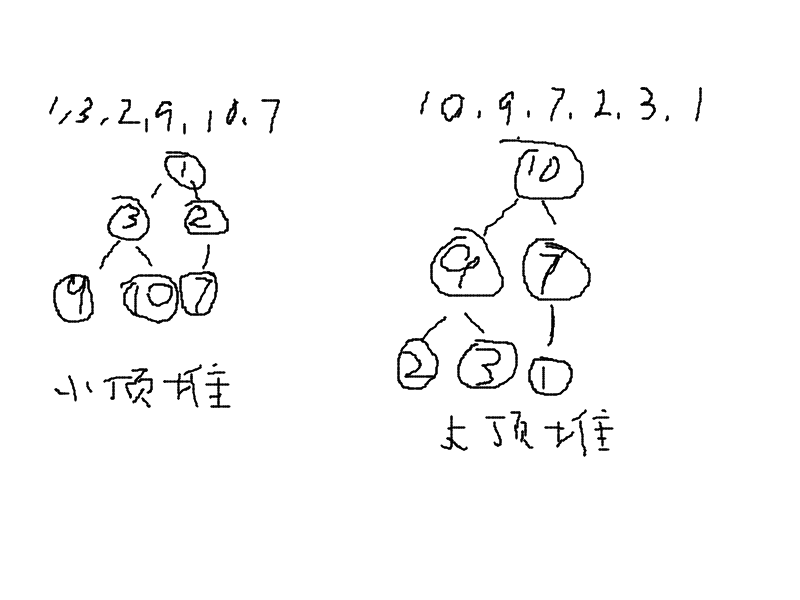
\includegraphics[scale=0.4]{./pic/tree-06.png}

		堆是完全二叉树。

		\textbf{堆排序}
		
		堆排序的思想是:

		1、首先对数组进行初始化,将其变成堆,
		
		2、然后取出堆顶元素,输出,将最后一个元素与堆顶元素交换,数组数目减1
		
		3、对堆筛选。

		4、重复2,3,直到最后一个元素

		筛选就是将当前节点与左右子树比较,将当前节点值用孩子节点中较小的值替代。

		\begin{verbatim}
    void sort(T *data,int size){
      T tmp;
      int i;
      init(data,size);
      //pop first data ,swap last data to first 
      //and then shift it.
      //note :when pop data ,the size must -1.
      for(i=size-1;i>=0;--i){
        tmp=data[0];  //swap data 
        data[0]=data[i];
        data[i]=tmp;
        shift(data,0,i-1);//adjust size
      }
    }
    //筛选
    void shift(T *data,int k,int n){
      T x;
      int finish=0;
      int i=k;
      int j=2*k+1;
      x=data[i];
      while(j<=n && !finish){
        if(j<n && data[j]>data[j+1])//avoid j+1 exceed n,so j<n
          j++;
        if(x<data[j]){
          finish=1;
        }else{
          data[i]=data[j];
          i=j;//record last swap pos
          j=2*i+1;
        }
      }
      data[i]=x;
    }
    void init(T *data,int s){
      int i;
      size=s;
      head=data;
      int k;
      k=size-1;
      for(i=size/2-1;i>=0;i--){
          shift(data,i,k);
      }
    }
		\end{verbatim}

	\subsection{树与森林}
	\subsubsection{树的存储结构}



	\	
\section{图与贪心算法}
	\subsection{图的概念}
		与线性表的一对一,树的一对多的关系相比,图表示多对多的关系。

		线性表和树可以看成图的特例。

		图分为有向图和无向图。

		图用G=(V,\{E\})来表示,V代表点的集合,E代表边的集合。V=\{v1,v2...\},
		E=\{(v1,v2),(v2,v3),...\}。

		对于有向图:0<=e<=n*(n-1),对于无向图:0<=e<=n*(n-1)/2

		\textbf{图的度}
		\begin{itemize}
			\item 无向图:依附于顶点v的边的数目。
			\item 有向图:以顶点v为弧头的边的数目,称为入度($ID(v)$)。以顶点v为弧尾的边的数目,称为出度($OD(v)$)。$TD(v)=ID(v)+OD(v)$
		\end{itemize}

		\textbf{图的路径}

		从v到v‘之间的顶点的集合。

		路径上边的数目称为路径的长度。

		\textbf{图的连通}

		从顶点v到v’有路径,则称v到v‘是连通的。

		对于无向图中任意两点$V_i$与$V_j$是连通的,则称该图为连通图。

		对于有向图中任意两点$V_i$与$V_j$是连通的,则称该图为强连通图。

		\textbf{连通分量}

		无向图:无向图中极大连通子图,称为连通分量。

		有向图:有向图中极大强连通子图,称为强连通分量。

		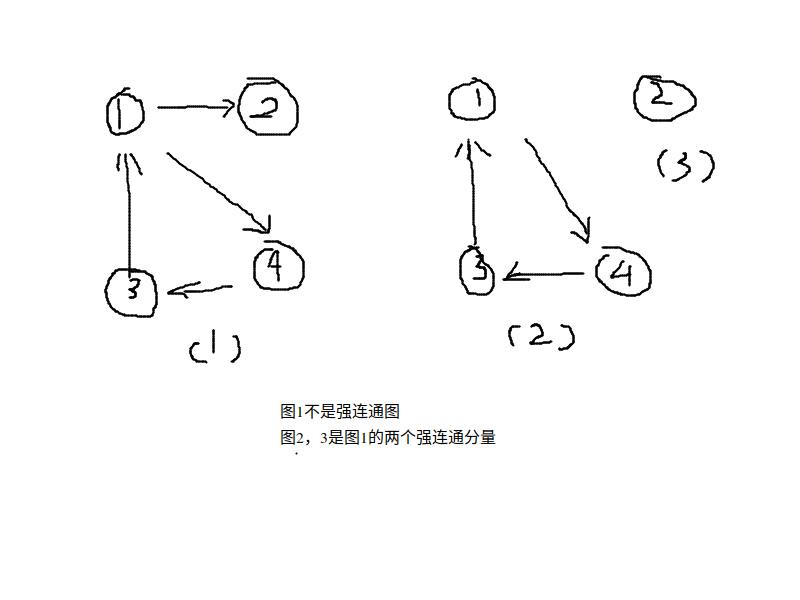
\includegraphics[scale=0.4]{./pic/graph-01.png}

		\textbf{生成树}

		假设图G是包括n个顶点的无向连通图,包括n个顶点,n-1条边的连通子图称为生成树。在生成树中加上一条边,则成为环。

		\textbf{子图}

		图中的一部分称为子图。

	\subsection{图的存储}
	\subsubsection{顺序存储(邻接矩阵)}
		如果图G(V,\{E\})有n个顶点,则邻接矩阵为n的方阵。

		其中:
		\[
			E(i,j)=
			\left\{
				\begin{array}{ll}
					1 & \textrm{当($V_i,V_j)$有边}\\
					0 & \textrm{当$(V_i,V_j)$无边}
				\end{array}
			\right .
		\]
		邻接矩阵即用点与点之间的关系表示边。
		V用一维数组表示。

		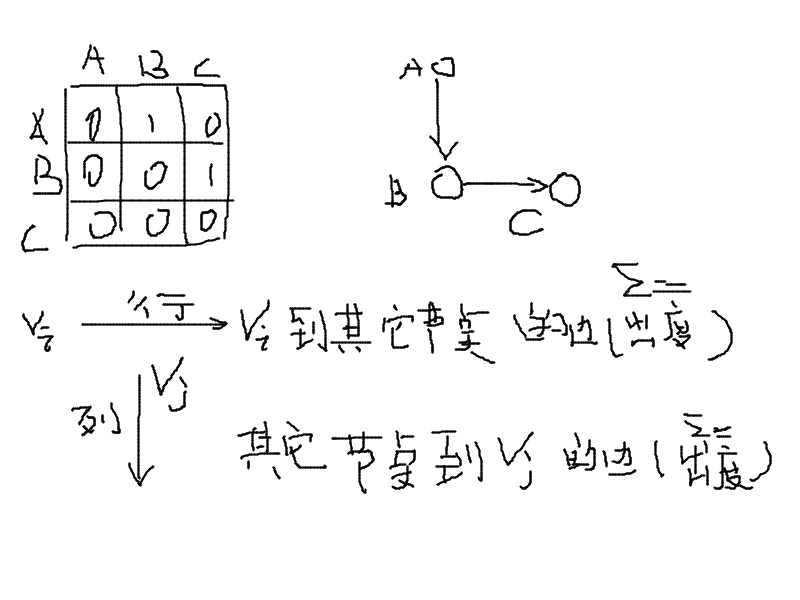
\includegraphics[scale=0.4]{./pic/graph-02.png}


		如果是带权图,可以:

		\[
			E(i,j)=
			\left\{
				\begin{array}{ll}
					W_{ij} & \textrm{当($V_i,V_j)$有边}\\
					\infty & \textrm{当$(V_i,V_j)$无边}\\
					0	& \textrm{自身}
				\end{array}
			\right .
		\]
		
		存储的数据结构如下:
		\begin{verbatim}
      #define MaxPoint 100
      template <class T>
      class MGraph{
        public:
          int edge[MaxPoint][MaxPoint];
          T data[MaxPoint];
          int n,e;//point and edges
      };
		\end{verbatim}
		\subsubsection{邻接表}
		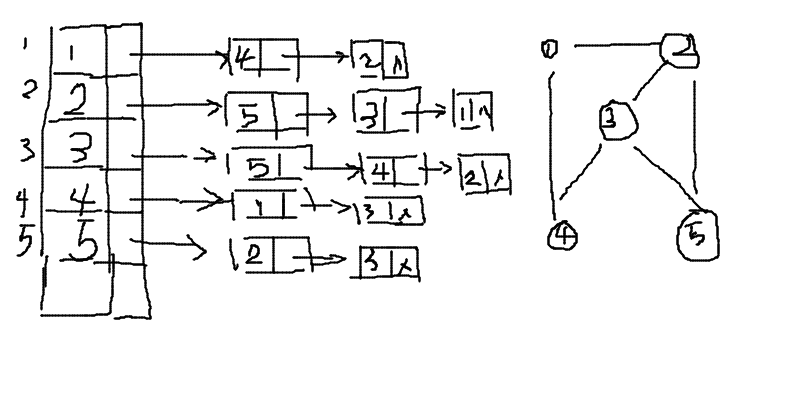
\includegraphics[scale=0.4]{./pic/graph-03.png}
		\begin{verbatim}
		struct adjnode{
		  int adj;
		  adjnode*next;
		};
		struct vexnode{
		   DataType data;
		   adjnode *first;
		}; 
		\end{verbatim}
		 
\section{动态规划}
%\end{CJK}
\end{document}
